\documentclass[12pt]{article}
\usepackage{lingmacros}
\usepackage{tree-dvips}
\usepackage{graphicx}
\usepackage[symbols,nogroupskip,sort=none]{glossaries-extra}
\usepackage[hidelinks]{hyperref}
\usepackage{geometry}
\usepackage[nottoc]{tocbibind}
\usepackage{enumitem}
\usepackage{amssymb}
\usepackage{listings}
\usepackage{algorithm}
\usepackage{algpseudocode}
\usepackage[utf8]{inputenc}
\usepackage{caption}
\usepackage{adjustbox}

\newgeometry{
top=0.75in,
bottom=0.75in,
outer=1.0in,
inner=1.5in,
}

\begin{document}


\begin{titlepage}
    
   \begin{figure}[t]
    \centering
    \begin{minipage}[t]{0.4\textwidth}
        \centering
        
\includegraphics[scale=0.9]{unibologo.png} % Replace with your image file
    \end{minipage}
    \hfill
    \begin{minipage}[t]{0.45\textwidth}
        \centering
        
\includegraphics[scale=0.8]{munerlogo.png} % Replace with your image file

    \end{minipage}
\end{figure}



     \centering
    \vspace*{4.5cm}
    
    {\huge \textbf{Product recognition on store shelves project}} % Huge, bold, centered title
    \vspace{2cm}
    
    
    {\begin{large}
AUTHORS:
\end{large} Iborra Lérida, Alex\\ \hspace{2.8cm} Fayetorbay, Orcun}
\vspace{1cm}

{\begin{large}
TUTOR:
\end{large} Di Stefano, Luigi} % Author's name
    \vspace{1.5cm}
     \vfill
    
    {\Large Università di Bologna \\ \vspace{0.4 cm} Motor Valley University of Emilia Romagna \\ \vspace{0.6 cm} Master Degree in Electronic Engineering for Intelligent Vehicles} % University name
   

\end{titlepage}




\newpage
\ \thispagestyle{empty}
\newpage

\pagenumbering{roman}
\tableofcontents


\newpage
\ \thispagestyle{empty}
\newpage 

\pagenumbering{arabic}

\section{Introduction}

This document shows the procedure followed to accomplish the project, its different main steps and difficulties that have arisen as well as their proposed solution.

\section{Problem description}

In this section the description of the problem is taken from the project proposal document:\\

Object detection techniques based on computer vision can be deployed in super market scenarios for the creation of a system capable of recognizing products on store shelves.\\

Given the image of a store shelf, such a system should be able identify the different products present therein and may be deployed, e.g. to help visually impaired costumers or to automate some common store management tasks (e.g. detect low in stock or misplaced products).

\section{Task definition}

The definition of the task is provided by the project proposal document:\\

Develop a computer vision system that, given a reference image for each product, is able to identify boxes of cereals of different brands from one picture of a store shelf. For each type of product displayed in the shelf the system should report:

\begin{enumerate}
	\item Number of instances.
	\item Dimension of each instance (width and height of the bounding box that enclose them in pixel).
	\item Position in the image reference system of each instance (center of the bounding box that enclose them in pixel).
\end{enumerate}

The task is also defined in three sub-tasks that increment the difficulty in each step:

\begin{itemize}
	\item \underline{Step A - Multiple Product Detection:} Develop an object detection system to identify single instance of products given: one reference image for
each item and a scene image. The system should be able to correctly identify all the product in the shelves
image. One way to solve this task could be the use of local invariant feature as explained in lab session 5.
	\item \underline{Step B - Multiple Instance Detection:} In addition to what achieved at step A, the system should now be able to detect multiple instance of the
same product. Purposely, students may deploy local invariant feature together with the GHT (Generalized
Hough Transform). More precisely, rather than relying on the usual R-Table, the object model acquired at
training time should now consist in vectors joining all the features extracted in the model image to their
barycenter; then, at run time all the image features matched with respect to the model would cast votes
for the position of the barycenter by scaling appropriately the associated joining vectors (i.e. by the ratio of
sizes between the matching features). 
	\item \underline{Step C (optional) - Whole shelve challenge:} Try to detect as much products as possible in this challenging scenario: more than 40 different product
instances for each picture, distractor elements (e.g. price tags…) and low resolution image. You can use
whatever technique to achieve the maximum number of correct detection without mistake.

\end{itemize}
\section{Solution development}
The project solution process will be explained along this section. 

\subsection{Step A - Multiple Product Detection:}
\label{StepA}

\subsubsection{Laboratory Session 5 procedure}
Following the description from the task, the procedure from Laboratory Session 5 is used.\\

It uses SIFT detector to find the keypoints for both scene and model images, and SIFT descriptor to generate the descriptors. To match the features FLANN is used, and after it Lowe's distance ratio test filters the matches. Finally, RANSAC is used to obtain a robust homography that translates keypoints from model image to scene image.\\

This scheme is modified to cycle through each scene image, and for each scene image to cycle through each model image to obtain the detections. Moreover, the original method to obtain a rectangular bounding box rather than a parallelepiped. These rectangles obtain the furthermost points in each direction from the matches, as seen here:

\begin{figure}[H]
        \centering
        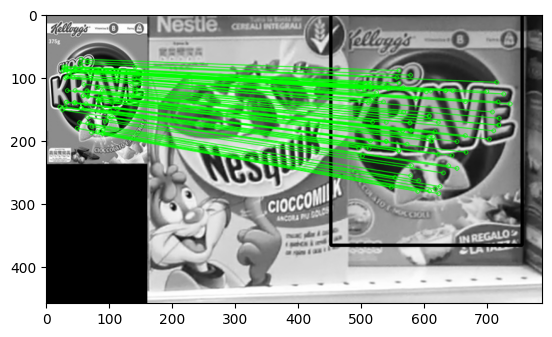
\includegraphics[scale=0.7]{boundingbox.png}
        \caption{Bounding box example}
\end{figure}

\subsubsection{Naive approach}

By following Laboratory Session 5 procedure without any addition, the results are not satisfactory. To understand this, it is necessary to know that SIFT works with grey scale images and finds features regardless of colour. As there are similar boxes that only change colour in some regions, these get confused by the algorithm\\

In this approach there is one degree of freedom: the minimum Lowe filtered matches necessary to consider a feature detection, but either higher or lower values do not reach a good solution as similar shaped cereal boxes get misinterpreted easily without the notion of colour.\\

For instance, in the first scene image, the two Krave models are very similar in shape but not in colour:

\begin{figure}[H]
        \centering
        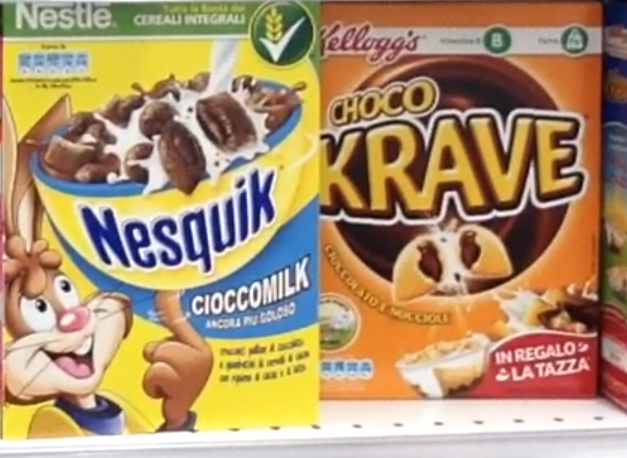
\includegraphics[scale=0.28]{e1.png}
        \caption{First scene image}
\end{figure}

\begin{figure}[H]
        \centering
        
\includegraphics[scale=0.062]{1.jpg}
        
\includegraphics[scale=0.52]{11.jpg}
        \caption{Krave models}
\end{figure}
 
 The two are identified with a similar number of filtered matches, as seen here they are labelled as Product 2 and Product 3:
 
 
 \begin{figure}[H]
        \centering
        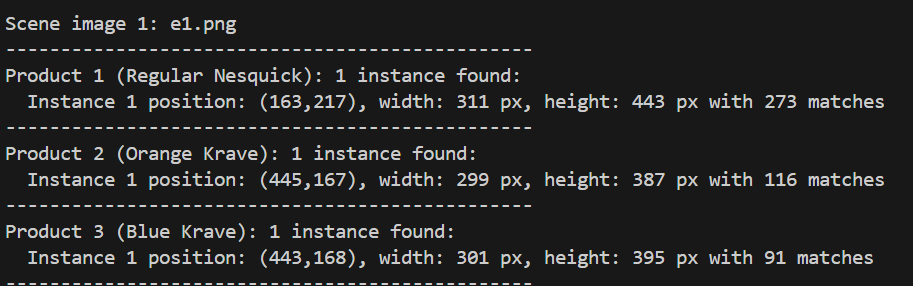
\includegraphics[scale=0.40]{naiveapproachoutput.png}
        \caption{First scene image}
\end{figure}


\subsection{General conditions}

In this section the relationship between client and contractor is detailed. 

\subsubsection*{Client functions}
The responsibilities that lie on the client are the following:

\begin{itemize}
	\item Mathematical model of the aircraft, including geometric, aerodynamic and propulsive information required to use control theory on it.
	\item Simulink\textsuperscript{\textregistered} model of the aircraft to be able to perform Software in the Loop (SIL) simulations.
	\item Regular implementation of the autopilot.
	\item Control specifications of the desired experimental implementation.
\end{itemize}

\subsubsection*{Contractor functions}
The responsibilities that lie on the contractor are the following:

\begin{itemize}
	\item Accomplish the different sections of the project with good engineering practices and provide the documents indicated in section \ref{documents}
\end{itemize}

However, as the dynamic model is a responsibility of the client, the contractor cannot guarantee its exactitude or the correct behaviour of the control.

\subsection{Conditions of the project accomplishment}


\subsubsection*{Project submission}
All of the output of the project, including documents specified in section \ref{documents}, and generated code, will be submitted to the client.\\


The code will be functional without the need of modifications or corrections, and will be properly commented for easy comprehension in case of future extensions of it. In case there is dissatisfaction of the final result by the client, modifications of it can be requested as long as it lies inside the project specifications. As previously stated, the dynamic model or experimental control specifications are responsibilities of the client. In case of dissatisfaction regarding these aspects, it is not the contractor responsibility to modify these.\\


For the project output to be replicated in other computer system, the required programs and tools will not be provided by the contractor. Instead, these will be detailed in section \ref{pliegotec}.

\subsubsection*{Deadline and time extensions}

The project deadline is agreed between both sides of the contract. It is detailed in section \ref{pliegotec}, where the different stages of the development are also mentioned. If it is requested by the client, it will be needed to provide written evidence of it.\\


If beginning or ending a project section inside the deadline is not feasible due to force majeure, a time extension will be provided for the sake of the contract. This time extension will be agreed between both sides of the contract.

\subsection{General economical conditions}

This section will detail the economical conditions of the project. The Costs document will provide the complete version of this section.

\subsubsection*{Prices}

For price calculations three different aspects are being considered:

\begin{itemize}
	\item \underline{Direct costs:} they include the labour cost, tools, material and software licenses.
	\item \underline{General costs:} they include costs that are not considered in direct costs, such as energetic, reparation or maintenance costs. These are considered to be 15\% of the direct costs.
	\item \underline{Industrial benefit:} it is the economic surplus obtained by a business after eliminating costs associated to production and distribution of goods or services. They are considered to be 6\% of the direct costs.
\end{itemize}


\section{Technical terms of reference}
\label{pliegotec}

\subsection{Motivation}

This section is responsible for describing the materials and tools used for the development of the project, which, due to the project nature, will include software licenses. Moreover, the terms of use of these are also described.

\subsection{Materials and tools conditions}

The materials and tools used are the different software programs needed for the code development and simulation. The terms of use of each of them are described:

\begin{itemize}
	\item \underline{MATLAB\textsuperscript{\textregistered} and Simulink\textsuperscript{\textregistered}:} For the former, version R2023b is used, and for the latter it is version 23.2. In addition, to be able to perform the required simulations, the following toolboxes are required, all with version 23.2:
	
	\begin{itemize}[label=\scalebox{0.5}{$\blacksquare$}]
	    \item Aerospace Blockset
	    \item Aerospace Toolbox
	    \item Control System Toolbox
	    \item Symbolic Math Toolbox
	\end{itemize}	

MATLAB is not open-source, it is a commercial software product that requires a paid license to use. Special academic licenses are available for students and educators at a discounted rate. These licenses may have additional restrictions, such as non-commercial use only. In this case, an educational version is used.


	\item \underline{QGroundControl:} it is a software dedicated to plan an autonomous mission , communicate with the autonomous aircraft, and visualize the environment in a simulation or real mission. The source code of QGroundControl is dual-licensed under Apache 2.0 and GPLv3 (or later), the artwork/images are licensed under CC by SA. The version being used is v4.3.0.
	
	
	\item \underline{PX4 source code:} It is an open-source flight control software for drones and other unmanned vehicles. It is the base code frame of the autopilot of the aircraft which will be modified to obtain an experimental version compatible with the regular implementation. PX4 is distributed under the BSD 3-Clause License. This is a permissive open-source license that allows for free use, modification, and distribution of the software, with minimal restrictions. The main conditions are that the original copyright notice, list of conditions, and disclaimers must be retained in all copies or substantial portions of the software. The version used is v1.14.0.
	

	\item \underline{Microsoft Visual Studio Code (VS Code):}  It is a free, open-source code editor developed by Microsoft. It is used to modify the PX4 source C++ code and develop the experimental control. Visual Studio Code is distributed under the Microsoft Software License Terms. The source code for Visual Studio Code is available on GitHub under the MIT License, which allows for free use, modification, and distribution of the source code. However, the official binary distributions provided by Microsoft come with a proprietary license that includes additional terms and conditions, particularly around redistribution and usage. The version used is 1.91.0.

	\item \underline{Texmaker:} It is a free, cross-platform LaTeX editor, which is the software used to create the documents of the project. Texmaker is distributed under the GNU General Public License (GPL) v2. This license allows users to freely use, modify, and distribute the software, provided that any distributed versions or derivative works also come under the GPL. The version used is 5.1.4.
	
	\item \underline{MiKTeX:} It is a distribution of the TeX/LaTeX typesetting system. It includes a package manager that automatically installs missing packages from the Internet. It is required for Texmaker to work, so the project documents also rely on this software. MiKTeX is distributed under the MiKTeX Project Public License, which is similar to the LaTeX Project Public License (LPPL). The source code for MiKTeX is available, and users can contribute to its development. The version used is 4.12.

\subsection{Description of tools usage}

This section provides the link between the procedures and tools needed for the project accomplishment:

\begin{itemize}[label={$\bullet$}]
	\item \underline{Modification of PX4 standard code and implementation of LQR algorithm code:} Using Microsoft Visual Studio and PX4 software, the C++ PX4 code is modified to suit the experimental LQR code and allow the different implementations to be switched from QGroundControl console.

	\item \underline{Aircraft dynamic model linearization and LQR parameter calculation:} the model is implemented in Simulink\textsuperscript{\textregistered} making use of the Aerospace Toolbox, Aerospace Blockset, Symbolic Math Toolbox and Control System Toolbox. The implementation is based on Bryan equations which approximate the behaviour of the flight of an aircraft. It is linearized and then using MATLAB\textsuperscript{\textregistered} the LQR parameters are calculated. Then, using Microsoft Visual Studio and PX4 software they are implemented in the code.
	
	\item \underline{Software in the Loop simulation:} the purpose is to run the experimental code and check that the original implementation works as well. With the Simulink\textsuperscript{\textregistered} model connected to QGroundControl, the mission is planned, launched and monitored. In this scenario, the regular and experimental implementations can be switched.
	
	
	\item \underline{System validation:} by looking at the error between the desired trajectory and the followed one from QGroundControl, the system performance is assessed.
\end{itemize}

\subsection{Final checks and adjustments}

Upon completion of project components, the client may assess the developed simulation system through testing with various autonomous missions. If the results of these tests are unsatisfactory, the client may request modifications to the simulation system, always falling between the project scope. This phase corresponds to the final adjustments of the project. Ultimately, the client will receive all documentation generated throughout the project, along with the code developed for each component, as per the terms of execution.

\end{itemize}


\newpage
\ \thispagestyle{empty}

\end{document}